\documentclass[12pt]{article}

%------------ PACKAGES ----------
\usepackage{mathtools}
\usepackage{csquotes}
\usepackage{graphicx}
\graphicspath{ {./figures/} }
\newcommand{\bigO}{\mathcal{O}}

%------------ MARGINS ----------
\addtolength{\oddsidemargin}{-.875in}
\addtolength{\evensidemargin}{-.875in}
\addtolength{\textwidth}{1.75in}
\addtolength{\topmargin}{-.875in}
\addtolength{\textheight}{1.75in}

%------------ TITLE INFO ------------
\title{Portfolio Optimization Using Geometric Mean, Risk Correlation 
    \& Multi-Variable Genetic Algorithms}
\author{Alex Lewis
\and {\small Supervisor:} Shan He}
\date{\today}

%------------ START DOCUMENT ----------
\begin{document}
\maketitle

\section{Abstract}

    TODO: its like a conclusion, but at the beginning

\pagebreak
\subsection{What is Portfolio Optimization}

    TODO

    \cite{Markowitz}

\subsection{Kelly Criterion}

    Kelly criterion is a well known concept for the most optimal way to grow a budget from a 
    given gamble. In the case where there is a positive expectation gamble, then using the 
    Kelly criterion is mathematically proven to be optimal. Based on the paper which under
    the guise of networking formally defines the optimal growth rate of a betting function
    with a fixed probability and payout.

    \begin{equation}\label{eq:KellyOriginal}
        k = \frac{(b \times p - (1 - p))}{b} 
    \end{equation}

    where:
    \begin{flalign*}
        k &= \text{The best size as a fraction of your portfolio} &&\\
        b &= \text{The net odds on the wager. i.e. your win } b + \text{ wager staked} &&\\
        p &= \text{The probability of winning} &&
    \end{flalign*}

    The equation \ref{eq:KellyOriginal} is from the famous paper by Kelly in 1956 \cite{Kelly}.
    Much work has been done to adapt the formula and make it more relevant to current economics.
    Firstly the equation \ref{eq:KellyOriginal} has one clear difference to real stocks and 
    investment which is that you are assumed to lose 100\% of your wager upon a loss. Which 
    while technically true in the worst case for a stock or bond investment. Is more often than 
    not, you lose a percentage of your initial investment. Typically you lose a smaller
    percentage than 100\%. Hence there is an adapted formula: 
    {(From the article by Alon\cite{Alon})}

    \begin{equation}\label{eq:KellyCorrect}
        k = \frac{p}{L} - \frac{1 - p}{W}
    \end{equation}

    where:
    \begin{flalign*}
        k &= \text{The best size as a fraction of your portfolio} &&\\
        L &= \text{The amount of money lost if its a loose result} &&\\
        W &= \text{The amount of money won if its a win result} &&\\
        p &= \text{The probability of winning} &&
    \end{flalign*}

    Equation \ref{eq:KellyCorrect} is adapted specifically for trading and modeling stocks.
    And, more precisely, it simply splits the \(b\) from Kelly's equation into its
    constituent parts, winning and losing.

\subsection{Kelly Criterion Application \& Assumptions}

    Kelly Criterion as concept is a great theoretical achievement, such a simple formula so
    perfectly describes how to play a system in order to gain the most from it. But alas
    stocks and trades are themselves not a repeatable and positive mathematical expectation
    game. Hence why we need to adapt the equations so that we can try to apply them to the
    real world.

    A big assumption which is being made from now on, by other papers - sometimes implicitly,
    is that we can model a stock as random variable. And this is a large assumption. It
    implies that from past data we can use this to construct a model which will be able
    to tells the probabilities associated with different outcomes of future events. Unlike
    in an actual variable, which once defined will always function the same. A stock will
    depend upon its past data to define its functionality.

    This furthermore means that as we gain new data, our model is constantly shifting.
    We do not have a fixed way to tell us probabilities of all future outcomes.
    To top this, we made another assumption: That its feasible to use past data to predict
    future events.

    This line of thinking has been criticized by the famous book "A Random Walk Down
    Wall Street" by Burton Malkiel \cite{BurtonMalkiel} it uses
    key economic historical events and many studies to describe how investing and trading are
    a futile game, compared to compound interest, or using an Index like S\&P 500. Which
    simply is a summation of the top 500 stocks in the US stock market.

    Instead of applying mathematics and statistics to your stock purchasing its contrary the 
    very nature of randomness, which is that humans look for patterns in all things. True 
    randomness seems to be against the very nature of what it is to be human, which is why
    there is still contention as to the ideas in the book. The idea that if you examine stock
    prices in a given period you can always find a system that would produce a positive return.

    A system which will always work and produce a positive return, and be mathematically sound. 
    I.e. it will work infinitely. Is an impossibility. We do not have an infinite amount of
    time to test our systems on infinite data.

    However, as much as I like the argument presented in the book and the complete contrast to 
    statistically minded way to analyze stocks. Ultimately a stock is buying a piece of an 
    actual business something which is valued on how it provides a product or service. And 
    looking back at businesses it becomes easier to see how the value of its stock is directly 
    related to the people in it, manning the ship.

    And for me, the only way to me to reason to myself that statistics, and analysis are still 
    useful. Is that a market is a system of people, which is something I don't believe we will 
    ever fully understand. But, statistics and short term analysis can give us insights as to 
    how it might work. It's too easy - for me at least - to accept that we our powerless and 
    nothing we can do in the long run will change that we can't beat randomness. Hence why
    trying to 'game' the system by using short term analysis to find businesses which happen
    to be doing well right now, for short term returns, is the only option we have against
    randomness.

\subsection{Optimal \(f\)}

    \begin{displayquote}[Ralph Vince \cite{Ralph}] \textit {
        For any given independent trials situation where you have an edge (i.e. positive 
        expectation) there exists an optimal fixed
        fraction (f) between 0 and 1 as a divisor of your biggest loss to bet on each event.
    } \end{displayquote}

    As it turns out this optimal \(f\) is similar to what Kelly describes in his paper. 
    And as Ralph proceeds, he explains how Kelly criterion is a perfect solution for 
    fixed size gambles with fixed wins and losses.

    But then the book reaches the a different conclusion, it goes on to state that trades where 
    the win or loss is always changing {(like the stock market)} then Kelly formula does find
    the correct optimal \(f\).
    So instead the book proposes finding the optimal \(f\) by instead using the geometric
    mean. \emph{Aside: We can use the estimated geometric mean because it is basically the
    same, while being much less computation}:

    \begin{equation}\label{eq:TWR}
        TWR = \displaystyle\prod^{N}_{i=1}1 + f \times \frac{- trade_i}{biggest loss}
    \end{equation}
    \begin{equation}\label{eq:GeoMean}
        Geometric Mean = exp(\frac{1}{N} \times Ln(TWR))
    \end{equation}

    where:
    \begin{flalign*}
    f &= \text{The optimal f} &&\\
    N &= \text{The number of trades} &&\\
    trade_i &= \text{The profit loss of the } i^{th} \text{ trade from the set of trades} &&\\
    biggest loss &= \text{The biggest loss from the set of trades} &&\\
    exp(x) &= \text{The exponential function} &&\\
    Ln(x) &= \text{The natural logarithm function} &&
    \end{flalign*}

    Equation from Ralph Vince's book\cite{Ralph}.
    To maximize our profit from a set of trades we want to optimize for the highest possible 
    geometric mean. Since \(f\) is a free standing variable which cannot be made the subject 
    of the equation we can only use iteration to find a good estimate. Or genetic algorithms
    as explained later.


\subsection{Portfolio's Compared to Single Stocks}

    Its a classical way of thinking to also consider diversification
    of your investments. Intuition tells us a single stock with a calculated optimal \(f\) that predicts
    good results, may still have "unlucky streaks" in which you can run out of money before
    your luck turns. Therefore we want a way to reduce our \(f\) by the correct amount
    to account for large streaks. Then use the left over unused money to invest in
    another (ideally uncorrelated) stock.

    This complicates the problem of finding optimal \(f\)'s for a set of stocks. As we
    need to find a set of \(f\)'s for each stock, to best diversify our portfolio, so
    its most resistant to unlucky streaks. While still producing good geometric growth.

    Thinking of the optimal \(f\) as a single point, inside a space of trades/bets. When we have 
    only a single trade/bet, we are doing calculations in a 2D space, and we have a line which 
    represents out optimal \(f\). However as the number of trades/bets increases we gain
    another dimension for each one.

    Therefore instead a \(f\) which lies on a line, it lies on a plane, or a 3D object, 
    and etc. If the \(f\) suddenly becomes a multi variable coordinate which must be 
    exactly correct. If a single axis is out then you can miss the hill of positive 
    growth, even if every other axis lined up.

    This means we need to define a new function to find the individual \(f\)'s for all the bets,
    but with relation to each other. We cannot compute each optimal \(f\) for every stock
    independently.


\subsection{Risk}

    Linking back to Kelly Criterion, the riskiness of a random variable is accounted for
    when use Kelly's formula, equation \ref{eq:KellyCorrect} needs no further calculations
    to account for how risky the variable is. And this is also true of geometric mean growth
    for stocks. The geometric accounts for the variance in the data of a single stock. As the
    equations \ref{eq:TWR} \& \ref{eq:GeoMean} are accounting for risk implicitly.

    But we need a new calculation to find the risk of the portfolio. And furthermore we would
    like a way to correlate stocks together so that we can more wisely spread our money.

    TODO: Drawdowns - why we want to find the overall risk
    TODO: Maybe risk of ruin talk?


\subsection{Mathematical Definition}

    Given the motivation from our the above sections, we would now like to formally define our
    evaluation function for how well a portfolio performs given a set of \(f\)'s. Which describes
    how we spread our money over a set of stocks.

    \begin{equation}\label{eq:G}
        G(f_1...f_m) = \left( \displaystyle\prod^{m}_{k=1} HPR_k \right) ^{ \left( \displaystyle\frac{1}{\sum^{m}_{k=1}Prob_k} \right)}
    \end{equation}
    \begin{equation}\label{eq:HPR_k}
        HPR_k = \left( 1 +  \displaystyle\sum^{n}_{i=1} f_k \times \frac{- PL_{k,i}}{BL_k} \right) ^{Prob_k}
    \end{equation}
    \begin{equation}\label{eq:Prob_k}
        Prob_k = \left( \displaystyle\prod^{n - 1}_{i=1} P(i_k | j_k)\right)^{\frac{1}{n - 1}}
    \end{equation}

    where:
    \begin{flalign*}
    n &= \text{The number of trades or bets in the } k^{th}\text{set} &&\\
    m &= \text{The number of stocks} &&\\
    f_k &= \text{The optimal } f \text{ for that }k^{th} \text{ set, where } f > 0 &&\\
    PL_{k,i} &= \text{The outcome for the } i^{th} \text{ trade or bet associated with the } 
        k^{th} \text{ set} &&\\
    BL_k &= \text{The worst trade or bet for the } k^{th} \text{ set} &&\\
    P(i_k | j_k) &= \text{Roughly it is the risk of }i^{th} 
        \text{ trade or bet associated with the } k^{th} \text{ set given the risk of the } &&\\
        & j^{th} \text{ trade or bet associated with the } k^{th} 
        \text{ set. Which is easy to calculate for coins, but I will explain} &&\\
        & \text{later how it is calculated for actual stocks} &&
    \end{flalign*}

    This equation is also from Ralph's Book \cite{Ralph}. Which is an execellent starting point,
    but it needs to be adapted to include this idea of correlation among stocks. And furthermore
    it needs to be decoupled, so that the risk of the overall stock is also found. The motivation
    for such a thing, is becuase of the nature of how this equation is solved. Which is explained
    later.


\subsubsection{Calculating Risk}

    Here we are actually constructing the risk calculation for a stock in a more concrete form.
    So must operate under some assumptions and natural patterns of a stock. 

    Proposed Model of a Stock: 
    \begin{itemize}
        \item{Open {\&} Close values for a given arbitrary time period}
        \item{A ratio of correlation to other stocks}
        \item{Holes of Open {\&} Close values may occur}
    \end{itemize}

    Calculating the profit{\/}loss of a stock at time period is now trivial and useful.
    Renaming the change in value at each time period \(i\) to \(PL_i\) we can find
    statistical facts about the stock.

    \begin{align}
        \text{mean: }
            \mu &= \frac{\sum^{i}_{n=1} PL_n}{i} \label{eq:StockMean} \\
        \text{variance: } 
            \sigma^2 &= \frac{\sum^{i}_{n=1} (PL_n - \bar{PL})^2}{i} \label{eq:StockVar}
    \end{align}

    Using this data we can transform a stock into a distribution which we can use to estimate
    the likely hood of the next \(PL_i\) being above a certain value. In our case we transform
    the normal distribution using equations \ref{eq:StockMean} and \ref{eq:StockVar} to find
    the mean and variance of the stock, and hence change the normal distribution. Then it is
    simple enough to use tables to find probabilities we want.

    \begin{equation} \label{eq:StockProb}
        P (PL) = \big( PL \sim \Phi(\mu, \sigma^2) \big) > 0
    \end{equation}
    
    where:
    \begin{flalign*}
    PL \sim \Phi (\mu, \sigma^2) &= \text{The cumulative normal distribution, adjusted to the mean } \mu \text{ and variance } \sigma^2 &&\\
    \text{ of the stock } PL\\
    \end{flalign*}

    Since calculating \(\Phi (\mu, \sigma^2)\) is incredibly hard to calculate and
    a perfect value isn't critical, we can settle for using tables as a close enough
    estimate.

    Accounting for 'holes' in the data, and the fact that older data may not be as relevant. Is
    currently overlooked if we were just going to implement these functions as our risk. The
    first change I am going to make is that we specify a time period and a range of time to
    take data from. This has multiple advantages, the first one being that we can choose to
    use only the most recent data about a stock. The second being that we can also choose
    how granular to make our risk calculation. It also builds directly into the algorithm
    the fact that the calculation will not use all available data from a stock, hence dealing
    with 'holes' at the same time.

    Now for the more complex part of the risk calculation, while the algorithm for it is
    simple, finding the data for it is a hard problem in itself. The equation
    \(P(i_k | j_k)\) hides the details behind the \(|\) symbol. Normally in statistics
    and probability of \(P(X | Y)\) means 'The probability of \(X\) given \(Y\) has occurred'
    which in a normal probability space is actually just a shorthand for:

    \begin{equation*}
        P ( X | Y ) = \frac{P(X \cap Y)}{P(Y)}
    \end{equation*}

    But in our stock based world we don't have an equivalent function \(\cap\) and hence
    we don't have the function \(|\) as well. The best we can do is assume that \(\cap\)
    is roughly equivalent to multiplying together the two stocks in question, and then
    assuming that \(\div\) is roughly equivalent to multiplying that by some amount of
    correlation. We cannot just multiply and divide as if they are independent probabilities as
    the first stock will just cancel out, hence doing nothing. So our function becomes:

    \begin{equation*}
        P ( X | Y ) = P ( X ) \times P ( Y ) \times C_{X, Y}
    \end{equation*}

    where:
    \begin{flalign*}
    C_{X, Y} &= \text{The pre-calculated correlation of stock } X \text{ to stock } Y&&\\
    P( X ) &= \text{The probability of } X \text{ given by the equation \ref{eq:StockProb}} \\
    \end{flalign*}

    However this doesn't work for lots of stocks as each probability is a smaller value 1, so
    when we times them all together, the value gets ever smaller regardless if each chance was
    actually quite high. For example, say we had 25 stocks, and each stock has a 0.9
    chance to make money, and for simplicity each correlation to every stock is 0.8:

    \begin{flalign*}
        \text{for all stocks } P &= 0.9 \times 0.9 \times 0.8 &&\\
        \text{hence } P &= 0.648 ^ {25} &&\\
        P &= 0.00001947041 \\
    \end{flalign*}

    So even in this example, with really high odds the overall chance of a single stock
    producing a likely chance. Therefore we need to use something which both preserve
    the chances of every stock, while taking into account how correlated something is.

    The solution is to use a weighted average over the stocks.
    And in the case where the correlation is negative we simply do \(1 - P(PL)\)
    when we calculate the average.

    \begin{equation} \label{eq:StockWeight}
        P ( X | Y ) = 
        \begin{cases}
            \displaystyle\frac 
                {P( X ) + (P ( Y ) \times C_{X, Y})}
                {1 + C_{X, Y}} 
                & \text{ if } C_{X, Y} >= 0\\
            \displaystyle\frac
                {P( X ) + ((1 - P ( Y )) \times - C_{X, Y})}
                {1 - C_{X, Y}} 
                & \text{ if } C_{X, Y} < 0
        \end{cases}
    \end{equation}

    Which brings us back to the claim that the algorithm is simple - all we do is find a
    weighted average of the stocks based on how correlated they are but, how do we find 
    and calculate good values for the table \(C\)? Some solutions are:

    \begin{enumerate}
        \item{Calculating the actual correlation, either Spearman's, or some other mathematical technique}
        \item{Using some form of NLP (Natural Language Parsing) to figure out how related the stocks are in the real world}
        \item{Grouping stocks by which industry they are in and assigning each group a correlation}
        \item{Assuming all stocks are independent}
        \item{Or a combination of all the above}\label{item:C}
    \end{enumerate}

    The answer to the question: how to find a good \(C\)? is probably worth its own paper, since
    its almost definitely point \ref{item:C}. Which requires a more complex analysis of the systems
    that make up a stock. At the end of the day the numbers we can gather about a stock never
    tell the full story. A stock is a part of a business, and a business is simply a is a
    group of people working together to sell a product or service to other people.
    And at the end of day using numbers to analyze how people will succeed in selling
    a product or service will always come up short compared to knowing and understanding
    the people who are ultimately doing the selling.

    For the sake of simplicity we will calculate the correlation as its mathematically defined.
    For example calculating the correlation between 2 stocks \(PL_1\) and \(PL_2\) is
    done as so:

    \begin{align}
        C_{PL_1, PL_2} = 
        \frac{
            \displaystyle\sum^{n}_{i=1} (PL_{1, i} - \bar {PL_1})(PL_{2, i} - \bar {PL_2})
        }{
            \sqrt{
                \displaystyle\sum^{n}_{i=1}(PL_{1,i} - \bar {PL_1})^2 
                \displaystyle\sum^{n}_{i=1}(PL_{2,i} - \bar {PL_2})^2
            }
        }
        \label{eq:Correlation}
    \end{align}

\pagebreak
\section{Finding \(f\)}

    Equations \ref{eq:G}, \ref{eq:HPR_k}, and \ref{eq:Prob_k} can be combined into one equation:

    \begin{equation}\label{eq:FullG}
        G(f_1...f_m) = \left(
            \displaystyle\prod^{m}_{k=1} \Bigg(
                1 + \displaystyle\sum^{n}_{i=1} f_k \times \Big(
                    \frac{- PL_{k,i} }{BL_k}
                \Big) 
            \Bigg)^{\Bigg(
                \displaystyle\prod^{n - 1}_{i=1} P(i_k | j_k)
            \Bigg) ^ {\frac{1}{n - 1}}} 
        \right) ^ {
            \left( {1 \div {\displaystyle\sum^{m}_{k=1}
                \Bigg( 
                    \displaystyle\prod^{n - 1}_{i=1}  P(i_k | j_k)
                \Bigg) ^ {
                    \frac{1}{n - 1}}
                }
            }
        \right)}
    \end{equation}

    where:
    \begin{flalign*}
    n &= \text{The number of trades or bets in the } k^{th}\text{set} &&\\
    m &= \text{The number of stocks} &&\\
    f_k &= \text{The optimal } f \text{ for that }k^{th} \text{set, where } f > 0 &&\\
    PL_{k,i} &= \text{The outcome for the } i^{th} 
        \text{ trade or bet associated with the } k^{th} \text{ set} &&\\
    BL_k &= \text{The worst trade or bet for the } k^{th} \text{ set} &&\\
    P(i_k | j_k) &= \text{The risk of }i^{th} \text{ trade or bet associated with the } 
        k^{th} \text{ set given the risk of the } &&\\
    & j^{th} \text{ trade or bet associated with the } k^{th} \text{ set. Defined by 
    equation \ref{eq:StockWeight}} &&
    \end{flalign*}

    TODO: Breif explanation why we can't solve this

\subsection{Decoupling \(G\)}

    In the original equation \ref{eq:FullG}, \(G\) is coupled with the risk of the portfolio
    by raising the inner calculation to 1 over the sum of all risks for every stock.
    There is another approach, which is to keep the two equations separate and use multi
    variable genetic algorithms to solve it. The motivation for this is to balance risk
    and reward independently, contrasting to the original \(G\) which lowers the gain
    by coupling it with the risk exponentially.

    \begin{equation}\label{eq:DecoupleG}
        G(f_1...f_n) = \displaystyle\prod^{m}_{k=1} \left(
                1 + \displaystyle\sum^{n}_{i=1} f_k \times \Big(
                    \frac{- PL_{k,i} }{BL_k}
                \Big)
            \right)
    \end{equation}

    \begin{equation}\label{eq:DecoupleR}
        R(f_1...f_n) = \displaystyle\prod^{m}_{k=1} \left(
                1 + f_k \times \Big(
                    \forall y \in m \to P(k|y)
                \Big)
            \right)
    \end{equation}

    where:
    \begin{flalign*}
    n &= \text{The number of trades or bets in the } k^{th}\text{ set} &&\\
    m &= \text{The number of combinations for all trades and bets} &&\\
    f_k &= \text{The optimal } f \text{ for that } k^{th} \text{ set, where } f > 0 &&\\
    PL_{k,i} &= \text{The outcome for the } i^{th} 
        \text{ trade or bet associated with the } k^{th} \text{ set} &&\\
    BL_k &= \text{The worst trade or bet for the } k^{th} \text{ set} &&\\
    P(k|y) &= \text{Equation \ref{eq:StockWeight} with the first stock } k \text{ correlated 
    with every other stock in the set } m &&
    \end{flalign*}

    Now we can use these functions separately to evaluate both risk and reward of the
    portfolio.

\pagebreak
\section{Solving \(f\) with respect to \(G\)}

    Intuition would suggest some form of iteration to check every combination of \(f\) to find
    the best performing \(f\). This has two major problems, the first being that we for every
    stock we add to our portfolio, we gain facortially many more combinations to check.

    \begin{equation*}
        \text{Number of combinations to check for: } \# F \text{ for } (f_1...f_m) = m!
    \end{equation*}

    Which in some senarios may be feasible, but becuase of our second major problem. The computation
    time of our evaluation functions. It becomes completly impossibile to actually calculate
    the mathematically correct solution in the lifetime of the universe.
    What follows is the Big \(\bigO\) \footnote{
        Originally defined by Bachmann \cite{Bachmann} to express orders of magnitude for 
        the time taken for computation
    } calculation for both problems:

    \begin{equation*}
        \text{Coupled: } \bigO (
            m! \times n^m
        )
    \end{equation*}
    \begin{equation*}
        \text{Decoupled: } \bigO (
            m! \times (n^m + (nm)^m)
        )
    \end{equation*}

    where:
    \begin{flalign*}
    n &= \text{The number of trades or bets in the stock} &&\\
    m &= \text{The number of stocks} &&
    \end{flalign*}

    The coupled equation \ref{eq:FullG} performs better as it can optimized by calculating
    equation \ref{eq:Prob_k} once, ahead of time. Whereas for the decoupled equations 
    \ref{eq:DecoupleG},
    \ref{eq:DecoupleR} it needs to calculate both, and equation \ref{eq:DecoupleR} has 
    considerably more
    calculations, which cannot be precomputed. But either way, both equations grow
    in number of calculation incredibly quickly, in fact too quickly to ever be
    solved by a pure mathematical solution. So we end up with an equation we want
    to solve, with no mathematically helpful properties (Differentailable being
    the most important), and it cannot be solved purely.

\subsection{Genetic Algorithms}

    \begin{displayquote}[Albert Bethke \cite{Bethke}] \textit {
        To find the point at which a real-valued function takes it maximal value ...
        If you don't know of any special properties of the function, then you
        should use a method which is more general like genetic algorithms.
    } \end{displayquote}

    Genetic algorithms (GA), first 
    discussed by John Holland \cite{Holland} in 1975, then developed by so many
    others, such as Melanie Mitchell \cite{Mitchell}, Kalyanmoy Deb \cite{KalyanmoyDeb},
    and Albert Bethke \cite{Bethke}, to name a mere few. are insipred by Darwinian
    principle of surivial of the fittest.
    First it is useful to define some biological terminology; in the context of
    genetic algorithms these terms are used in the same spirit as the real biology,
    but heavily simplfied. In an attempt to emulate thier nature as a living entity,
    while being computationally easier to process.

    \begin{itemize}
        \item{\textbf{Gene:} The encoding of a trait, and roughly it stores the current
            setting for the trait (e.g. eye colour, blue, brown, etc). There is a set
            from which any single gene can pull its data from. In nature its the chemical
            bases  of DNA}
        \item{\textbf{Genome:} The complete collection of all the genes is called a
            genome}
        \item{\textbf{Reproduction:} During reproduction each parent's genomes will be
            combined and crossed over creating a child which has a combination of
            the traits of its parents}
        \item{\textbf{Mutation:} During crossover there is a chance a single gene
            may be incorrectly copied, and mutate into a different gene}
        \item{\textbf{Fitness: } In nature the fitness of an animal determines
            its chances of surival and therefore its chance to pass on its genes
            and be the most successful animal. In GA the level of fitness is not assessed
            by nature, but by an \textbf{Objective} function}
    \end{itemize}

    The general procdeure of a GA is better explained with a diagram:

    \begin{figure}[h] % fig:GA
        \centering
        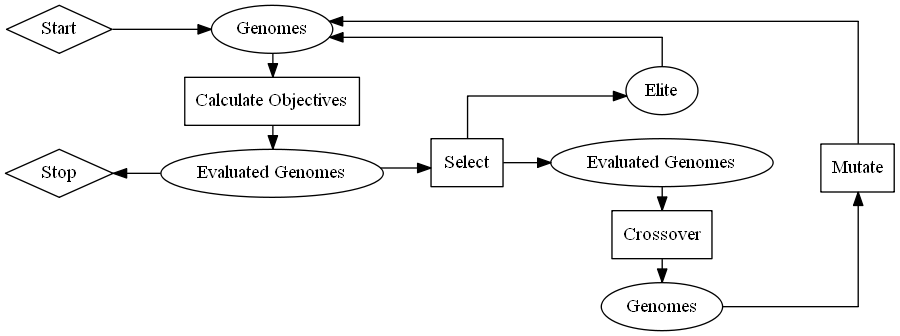
\includegraphics[width=\textwidth]{GA}
        \caption{"Life Cycle" of A Genetic Algorithm}\label{fig:GA}
    \end{figure}

    One note about figure \ref{fig:GA} is that the decision to go to the "Stop"
    state is determined by some outside factor i.e. execution time. Otherwise
    it repeats infinitly - just like real life. Applying this generic algorithm to 
    our specific problem. We simply need to
    define each state in this diagram in the context of our problem.

    The \textit{Genomes} state for our problem is the set of \(f\)'s. Each gene is an
    \(f\) for a specific stock. But we have addtional constraints, which is for 
    any genome \((f_1...f_m)\) made up of genes \(f_i\). The genome \textbf{must}
    abide by these laws:

    \begin{equation*}
        0 < \left(
            \displaystyle\sum^{m}_{i=1} f_i
        \right) <= 1
    \end{equation*}
    \begin{equation*}
        \forall f_i \in (f_1...f_m) \to \left(
            0 < f_i <= 1
        \right)
    \end{equation*}

    which more simply states, we can't bet more than our entire wealth over all the stocks or
    a negative bet. And on a single stock we can't place a negative bet more than our
    entire portfolio.

    The \textit{Select} state is a function which takes all pairs of evaluated genomes
    and thier fitness. And based on how well each genome performs, will cull the
    list of genomes to a smaller list. This smaller list is the list of genomes
    which act as parents for the next generation.

    The \textit{Elite} state is another output from the select function. Which is
    the most fit genomes have thier lifespan extended into the next generation.
    Importantly this elite population be very small, aswell as avoiding the
    chance to its genes to be destroyed by crossover and mutation. \cite{DeJong}
    This allows the best genome to always stay alive, and stops the GA from
    having to re-discover previously good results.

    The \textit{Crossover} state can simply be the same as any generic GA implementation,
    as we have no extra constraints to worry about. TODO: Explain crossover choice

    The \textit{Mutate} state needs to make sure it follows the same constraints as
    genomes states has to follow. Futhermore since this step is after crossover,
    any genomes which violate the laws will be fixed in this step. Other than this,
    mutation can be any generic GA mutation. TODO: Explain mutation choice

    Finally the \textit{Calculate Objectives} state, which is the final product of all our
    mathematical exploration. Here we have two options the single variable option: equation
    \ref{eq:FullG}, or the decoupled multi-variable option: equations \ref{eq:DecoupleG}
    and \ref{eq:DecoupleR}.

\pagebreak
\bibliographystyle{IEEEtran}
\bibliography{Report}

\end{document}